\subsection{Iterazione sul Prototipo e Realizzazione della Versione Web}

Dopo la revisione euristica sul prototipo Figma, è stata avviata la realizzazione della versione web definitiva.
Il prototipo ha rappresentato il punto di partenza per la struttura e la logica dei flussi, ma in questa fase l’attenzione si è concentrata sull’uniformità visiva, sulla chiarezza dei feedback e sulla robustezza dei meccanismi di interazione.

\subsubsection*{Uniformità visiva tramite PrimeVue}
Per garantire coerenza grafica e semplicità di manutenzione, il frontend è stato sviluppato utilizzando il framework \textbf{PrimeVue}.
L’adozione di questa libreria ha permesso di centralizzare le configurazioni di stile e di utilizzare componenti visivi coerenti in tutto il sistema.
Grazie a questa scelta, i popup, i pulsanti, le form e le finestre modali seguono lo stesso schema cromatico e tipografico, assicurando uniformità tra tutti i flussi applicativi.
Le differenze grafiche riscontrate nel prototipo, in particolare nei modali di conferma e negli alert, sono state eliminate, ottenendo un’interfaccia più pulita e coerente.

Inoltre, negli step di creazione di un annuncio sono state introdotte icone rappresentative per ciascuna fase del processo (es. dettagli, immagini, pubblicazione).
Questo accorgimento ha migliorato la corrispondenza tra sistema e mondo reale, rendendo il flusso più intuitivo e riconoscibile anche a colpo d’occhio.
\textit{Le Figure~\ref{fig:popup-login} e~\ref{fig:popup-conferma} mostrano i popup uniformati, mentre le Figure~\ref{fig:stepper-prima} e~\ref{fig:stepper-dopo} illustrano rispettivamente la versione dello stepper prima e dopo l’introduzione delle icone.}

\begin{figure}[H]
\centering

\includegraphics[width=0.8\textwidth]{Immagini/Expert Reviews/Figma/StepperCreazioneAnnuncio.png}
\caption{Stepper originale senza icone descrittive.}
\label{fig:stepper-prima}
\end{figure}

\begin{figure}[H]
\centering

\includegraphics[width=0.8\textwidth]{Immagini/Expert Reviews/Sito/StepperCreazioneAnnuncio.png}
\caption{Stepper aggiornato con icone rappresentative per ogni fase.}
\label{fig:stepper-dopo}
\end{figure}


\vspace{4pt}
\textit{(Figura~\ref{fig:popup-login}) mostra il popup di login con stile uniforme, mentre la Figura~\ref{fig:popup-conferma} illustra un esempio di messaggio di conferma.}

\vspace{4pt}
\textit{Le Figure~\ref{fig:popup-login} e~\ref{fig:popup-conferma} mostrano rispettivamente il popup di login e quello di conferma, uniformati nello stile PrimeVue.}

\begin{figure}[H]
\centering
\begin{minipage}[t]{0.48\textwidth}
    \centering
    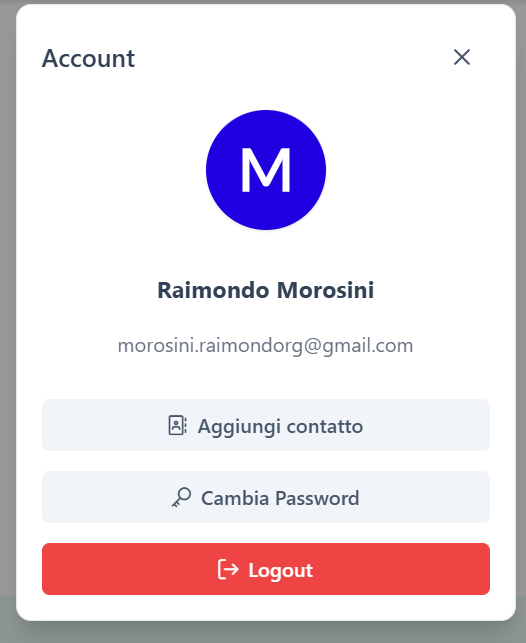
\includegraphics[width=\textwidth]{Immagini/Expert Reviews/Sito/PopupAccount.png}
    \caption{Popup di login con stile uniforme (PrimeVue).}
    \label{fig:popup-login}
\end{minipage}
\hfill
\begin{minipage}[t]{0.48\textwidth}
    \centering
    
\includegraphics[width=\textwidth]{Immagini/Expert Reviews/Sito/CreazioneAnnuncioConSuccesso.png}
    \caption{Esempio di popup di conferma operazione riuscita.}
    \label{fig:popup-conferma}
\end{minipage}
\end{figure}

\subsubsection*{Gestione degli errori e miglioramento del feedback}
Uno dei principali interventi rispetto al prototipo riguarda la gestione degli errori nel form di creazione di un annuncio.
Nel prototipo la validazione era presente ma meno visibile; nella versione web, per ogni step del processo, è stata introdotta una sezione evidenziata con sfondo rosso che riepiloga in modo chiaro tutti gli errori presenti.
In questo modo, l’utente può identificare immediatamente i campi errati senza doverli cercare manualmente, riducendo tempi e confusione.

\vspace{4pt}
\textit{(Figura~\ref{fig:errore-step}) mostra la nuova area di segnalazione errori all’interno dello step di creazione annuncio.}

\begin{figure}[H]
\centering
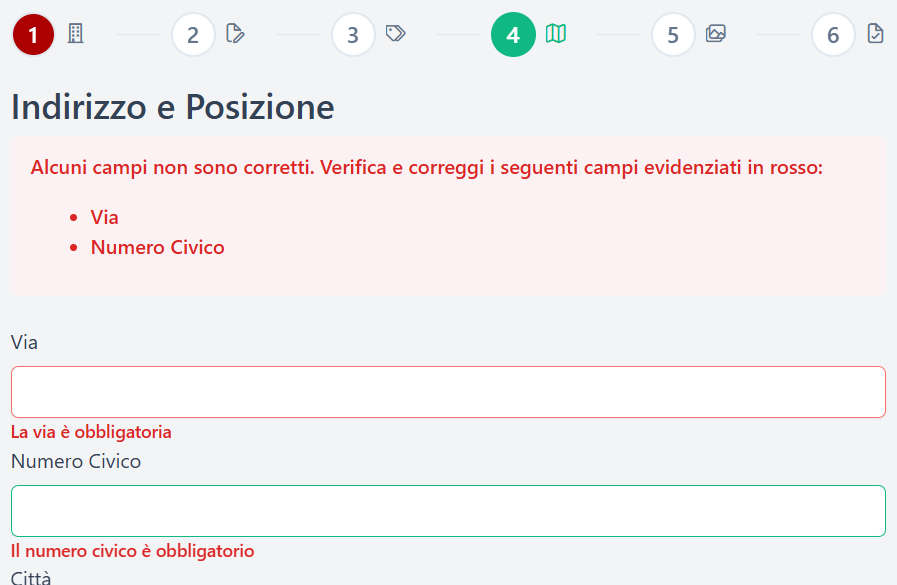
\includegraphics[width=0.8\textwidth]{Immagini/Expert Reviews/Sito/CreazioneAnnuncioConErrori.png}
\caption{Area di validazione con sfondo rosso nel form di creazione annuncio.}
\label{fig:errore-step}
\end{figure}

\subsubsection*{Conferme e messaggi di sistema}
Tutte le operazioni critiche o potenzialmente irreversibili (come eliminazione o pubblicazione) sono ora accompagnate da messaggi di conferma dedicati, garantendo un controllo maggiore da parte dell’utente.
Sono stati inoltre introdotti popup per notificare errori, conferme e caricamenti, tutti realizzati tramite componenti PrimeVue uniformi.

\vspace{4pt}
\textit{(Figura~\ref{fig:popup-errore}) e (Figura~\ref{fig:popup-success}) mostrano rispettivamente un messaggio di errore e una conferma di successo.}

\begin{figure}[H]
\centering
\begin{minipage}[t]{0.48\textwidth}
    \centering
    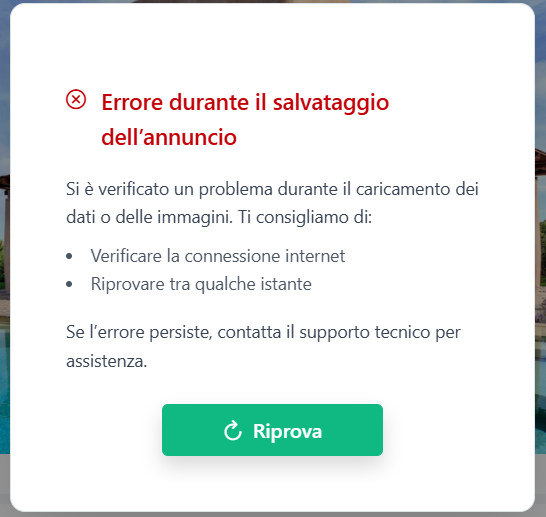
\includegraphics[width=\textwidth]{Immagini/Expert Reviews/Sito/CreazioneAnnuncioErrore.png}
    \caption{Esempio di popup di errore.}
    \label{fig:popup-errore}
\end{minipage}
\hfill
\begin{minipage}[t]{0.48\textwidth}
    \centering
    
\includegraphics[width=\textwidth]{Immagini/Expert Reviews/Sito/PopupRegistrazioneAccountGoogleGiaPresentepng.png}
    \caption{Esempio di stato di successo in un’operazione.}
    \label{fig:popup-success}
\end{minipage}
\end{figure}

\subsubsection*{Visibilità dello stato del sistema e animazioni}
Per migliorare la percezione di reattività, è stato aggiunto un indicatore di caricamento nelle fasi di attesa, come durante la ricerca di annunci o l’elaborazione di richieste.
A differenza del prototipo, dove si ipotizzava una progress bar, la versione web utilizza uno spinner circolare, più adatto per operazioni asincrone di durata variabile.
Lo spinner comunica all’utente che il sistema è attivo anche in assenza di un progresso misurabile, migliorando la trasparenza e riducendo l’ansia da attesa.

\vspace{4pt}
\textit{(Figura~\ref{fig:popup-loading}) mostra lo spinner di caricamento utilizzato nei popup.}

\begin{figure}[H]
\centering

\includegraphics[width=0.7\textwidth]{Immagini/Expert Reviews/Sito/CreazioneAnnuncioCaricamento.png}
\caption{Animazione di caricamento (spinner) durante operazioni asincrone.}
\label{fig:popup-loading}
\end{figure}

\subsubsection*{Sintesi dei miglioramenti principali}
La tabella seguente riassume le principali modifiche introdotte rispetto al prototipo Figma e i relativi benefici in termini di usabilità.

\begin{table}[H]
\centering
\setlength{\tabcolsep}{6pt}
\renewcommand{\arraystretch}{1.2}
\begin{tabular}{p{5cm} p{10cm}}
\hline
\textbf{Criticità nel prototipo} & \textbf{Soluzione implementata nella versione web} \\
\hline
Popup con stili differenti & Uniformati tramite componenti PrimeVue centralizzati \\
Assenza conferma creazione annuncio & Aggiunto popup di conferma prima della pubblicazione \\
Errori dispersi nel form & Introdotta sezione rossa riepilogativa per ogni step \\
Progress bar nei caricamenti & Sostituita con spinner per attese di durata variabile \\
Assenza icone negli step & Aggiunte icone descrittive per migliorare la comprensione visiva \\
Feedback visivo poco distinto & Differenziati colori per errori, successi e conferme \\
\hline
\end{tabular}
\caption{Sintesi dei miglioramenti principali introdotti nella versione web.}
\end{table}

\subsubsection*{Autovalutazione euristica della versione web}

È stata quindi condotta una nuova autovalutazione secondo i dieci principi di Nielsen, con l’obiettivo di verificare l’efficacia delle migliorie e individuare ulteriori aree di sviluppo.

\begin{table}[H]
\centering
\setlength{\tabcolsep}{6pt}
\renewcommand{\arraystretch}{1.2}
\begin{tabular}{p{0.4cm} p{4cm} p{1.5cm} p{7cm}}
\hline
\textbf{\#} & \textbf{Criterio} & \textbf{Valutazione} & \textbf{Motivazione sintetica} \\
\hline
1 & Visibilità stato & 2 & Spinner e messaggi di caricamento chiari in tutte le operazioni \\
2 & Corrispondenza mondo reale & 2 & Linguaggio coerente e icone aggiunte negli step migliorano la comprensione \\
3 & Controllo e libertà & 2 & Tutte le azioni critiche prevedono conferma e possibilità di annullamento \\
4 & Coerenza e standard & 2 & PrimeVue centralizza lo stile e uniforma i componenti grafici \\
5 & Prevenzione errori & 2 & Area rossa riepiloga errori per ogni step; validazione efficace \\
6 & Efficienza/flessibilità & 1 & Mancano shortcut, funzioni per utenti esperti e salvataggio bozza cross-device \\
7 & Chiarezza del contenuto & 2 & Testi sintetici e coerenti, layout leggibile anche su dispositivi diversi \\
8 & Supporto al riconoscimento & 2 & Navigazione intuitiva, icone e percorsi chiari tra le sezioni \\
9 & Feedback/Conferme & 2 & Popup coerenti per conferme, errori e caricamenti \\
10 & Aiuto/Documentazione & 0 & Assenti FAQ, onboarding e funzioni di accessibilità \\
\hline
\end{tabular}
\caption{Autovalutazione euristica della versione web secondo i principi di Nielsen.}
\end{table}

\subsubsection*{Analisi critica e prospettive di miglioramento}
La versione web rappresenta un’evoluzione matura e coerente del prototipo Figma, con un significativo miglioramento nella consistenza grafica, gestione degli errori e chiarezza dei feedback.
Tuttavia, l’analisi critica mette in evidenza alcune aree ancora aperte:
\begin{itemize}
\item \textbf{Accessibilità non implementata}: mancano funzioni per utenti con disabilità (navigazione da tastiera, supporto screen reader).
\item \textbf{Bozze non persistenti}: i dati sono salvati solo nel \textit{Pinia store} locale, quindi non recuperabili su dispositivi diversi.
\item \textbf{Mancanza di scorciatoie e funzioni avanzate} per utenti esperti.
\item \textbf{Assenza di FAQ o onboarding guidato} che agevolino la comprensione iniziale.
\item \textbf{Ottimizzazione mobile solo parziale}, soprattutto in visualizzazione verticale.
\end{itemize}